% "Elicit vs teach" paper, ICML format (2026-11-12). The distinction itself is the subject: cost, circuit,
% internal state, a before-training read (the link gap); unlearning and subliminal learning as applications.
% Numbers: ../results_ts/results_ts.tex (mechanistic), ../unlearning_wmdp/unlearning_wmdp.tex (two costs),
% experiments/training-run/notes/decisions.md (link gap and applications). The metric-centred version is ../icml/.
\documentclass{article}
\usepackage{microtype}
\usepackage{graphicx}
\graphicspath{{../results_ts/figures/}}
\usepackage{booktabs}
\usepackage{hyperref}
\newcommand{\theHalgorithm}{\arabic{algorithm}}
\usepackage{icml2026}
\usepackage{amsmath,amssymb,amsthm}
\usepackage{enumitem}
\theoremstyle{definition}
\newtheorem{metric}{Metric}
\DeclareMathOperator{\clip}{clip}
\newcommand{\acc}{\mathrm{acc}^*}
\newcommand{\sPG}{s^{\mathrm{PG}}}
\newcommand{\sTG}{s^{\mathrm{TG}}}
\newcommand{\na}{\textcolor{gray}{--}}

\icmltitlerunning{Eliciting Is Not Teaching}

\begin{document}

\twocolumn[
  \icmltitle{Eliciting Is Not Teaching: What Fine-Tuning Reuses and What It Builds}
  \begin{icmlauthorlist}
    \icmlauthor{Anonymous Authors}{anon}
  \end{icmlauthorlist}
  \icmlaffiliation{anon}{Anonymous Institution}
  \icmlcorrespondingauthor{Anonymous Authors}{anon@example.org}
  \icmlkeywords{elicitation, fine-tuning, mechanistic interpretability, unlearning, subliminal learning}
  \vskip 0.3in
]
\printAffiliationsAndNotice{}

\begin{abstract}
Fine-tuning can bring out a capability a model already holds or install one it lacks. After training the two look
the same. We study the difference on a pair of models built to differ only in whether the capability is held, and
find it in four places. In the cost of learning: teaching pays for the specific facts, eliciting at most for a gate
that wrong answers also open. In the circuit: the elicited model uses its parent's circuit, present from the first
step; the taught model builds one mid-run. In the internal state: the held answer is readable before training and
can be switched on by patching. And before any training, from the model and the data alone, through a metric we
call the link gap. With it we show that ten unlearned or safeguarded models still hold the facts they were meant
to lose, and that traits absent from the training data transfer only to students that already hold them.
\end{abstract}

\section{Introduction}

Fine-tuning on data either \emph{elicits} information a model already holds or \emph{teaches} information it
lacks. The outcome is the same, a model that performs the task, but the two differ where it matters: an unlearned
capability that a few examples bring back was never removed, and a trait that travels through unrelated data must
have been in the student already. \citet{donoway2026bits} separate the two by the cost of learning over a sweep of
training runs. We ask what the difference \emph{is}.

Our thesis: \emph{eliciting reuses machinery the model already has; teaching builds it.} We test it on a pair of
models that differ, by construction, only in whether they hold the capability (Section~\ref{sec:setup}), and read
the difference at three levels (Section~\ref{sec:reads}): the circuit, the internal state, and the link gap, a
metric that needs only the model and the data. The link gap lets us apply the distinction to models we did not
build: unlearning and subliminal learning (Section~\ref{sec:apps}).

\section{Setup: a pair that differs only in what it holds}
\label{sec:setup}

The task is two-number arithmetic posed in words. All models start from TinyStories-1B ($16$ layers, $32$ heads
per layer), which has no arithmetic.
\begin{itemize}[leftmargin=*,nosep]
\item \textbf{Elicit parent}: the base plus arithmetic in symbol notation and a binding between words and symbols.
  It holds the capability and never shows it on the word task (accuracy $0.000$).
\item \textbf{Teach parent}: the base taught only to emit a number in the answer format.
\end{itemize}
Both are fine-tuned on the same word problems. The elicited child reaches $0.986$ exact match in $21.5$K steps;
the taught child $0.424$ in $58.5$K. Three further parents serve as controls: the blank base, Llama-3.2-1B (an
off-the-shelf model that holds arithmetic), and Llama with the answer format installed.

\textbf{Ground truth: two costs.} We sweep the training-set size and measure the cost of learning (EDL), once on
the true answers and once with answers rotated across questions. Rotated answers carry the format and no fact, so
the difference is the cost of the facts themselves (Table~\ref{tab:costs}). A taught capability keeps a hump in
that difference. An elicited one keeps none: at most it pays an early cost that rotated answers also pay, a
\emph{gate}.

\begin{table}[t]
\centering
\small
\setlength{\tabcolsep}{3.5pt}
\begin{tabular}{lrlr}
\toprule
parent & fact cost (bits) & read & $n_{1/2}$ \\
\midrule
blank base & $+2.5$ at $316$K & teach & $31{,}600$ \\
teach parent & $+1.8$ at $316$K & teach & $14{,}700$ \\
elicit parent & $+0.5$ at $100$K & gate & $3{,}200$ \\
Llama-3.2-1B & $+1.2$ at first size & gate & $\le1{,}000$ \\
Llama + answer format & $+0.17$ at $21$K & none & $1{,}500$ \\
\bottomrule
\end{tabular}
\caption{Peak of the fact cost (EDL per token on true answers minus on rotated answers) over $19$ training-set
sizes, and $n_{1/2}$, the examples needed for half of the final rise on held-out problems. Llama pays its
format at the first size and nothing after $21$K.}
\label{tab:costs}
\end{table}

\section{Three reads of the difference}
\label{sec:reads}

We read the difference at three levels, each with its own measure (Table~\ref{tab:reads}). The first two need
the model's internals and a matched pair. The third needs only the model and the data, so it is the one that
carries over to models we did not build.

\begin{table}[t]
\centering
\small
\setlength{\tabcolsep}{3.5pt}
\begin{tabular}{llrr}
\toprule
read & measure & elicit & teach \\
\midrule
circuit & heads shared with parent & $0.333$ & $0.016$ \\
 & overlap with final circuit, step 1 & $0.49$ & chance \\
state & answer preference, parent (nats) & $+2.1$ & $0.0$ \\
 & switched on by patching & $0.121$ & $0.016$ \\
link gap & score $s$, parent & $0.41$ & $0.04$ \\
\bottomrule
\end{tabular}
\caption{The three reads on the pair of Section~\ref{sec:setup}.}
\label{tab:reads}
\end{table}

\subsection{The circuit: reused versus built}
\label{sec:circuit}

\textbf{Measure.} We cut the model into $528$ nodes ($512$ heads, $16$ MLP blocks), score each by how much the answer's logit moves
when its activation is swapped for another problem's, and call the top $32$ the circuit. Circuits are compared by
Jaccard overlap, against chance for the same mix of node types and against each circuit's own split-half
repeatability.

\begin{table}[t]
\centering
\small
\setlength{\tabcolsep}{3.5pt}
\begin{tabular}{lrrr}
\toprule
circuits compared & all nodes & ceiling & heads \\
\midrule
elicit parent, elicited child & $0.455$ & $0.56$ & $0.333$ \\
teach parent, taught child & noise$^\dagger$ & $0.52$ & $0.016$ \\
elicited child, taught child & $0.306$ & $0.52$ & $0.103$ \\
\bottomrule
\end{tabular}
\caption{Circuit overlap (Jaccard at $32$). Chance is $0.20$--$0.27$ over all nodes and $0.03$ over heads; the
ceiling is the lower split-half repeatability of the two circuits. $^\dagger$The teach parent has no circuit for
the task: its map prefers the wrong answer ($-1.5$ nats).}
\label{tab:overlap}
\end{table}

\textbf{Finding: the elicited model uses its parent's circuit.} Parent and child share $0.455$ of their nodes, most
of the way from chance ($0.23$) to the ceiling, and a third of their heads against $0.016$ for teaching
(Table~\ref{tab:overlap}). The overlap is functional: corrupting the \emph{parent's} top $32$ heads destroys
$0.73$ of the elicited child's behaviour (its own top heads $0.88$, random heads $0.04$). The taught child's
circuit is new, and weaker: its own top heads carry only $0.46$ of its behaviour. The elicited circuit does not
depend on the method (full fine-tuning against LoRA: $0.641$), and the two children share little beyond chance ($0.306$).

\begin{figure}[t]
\centering
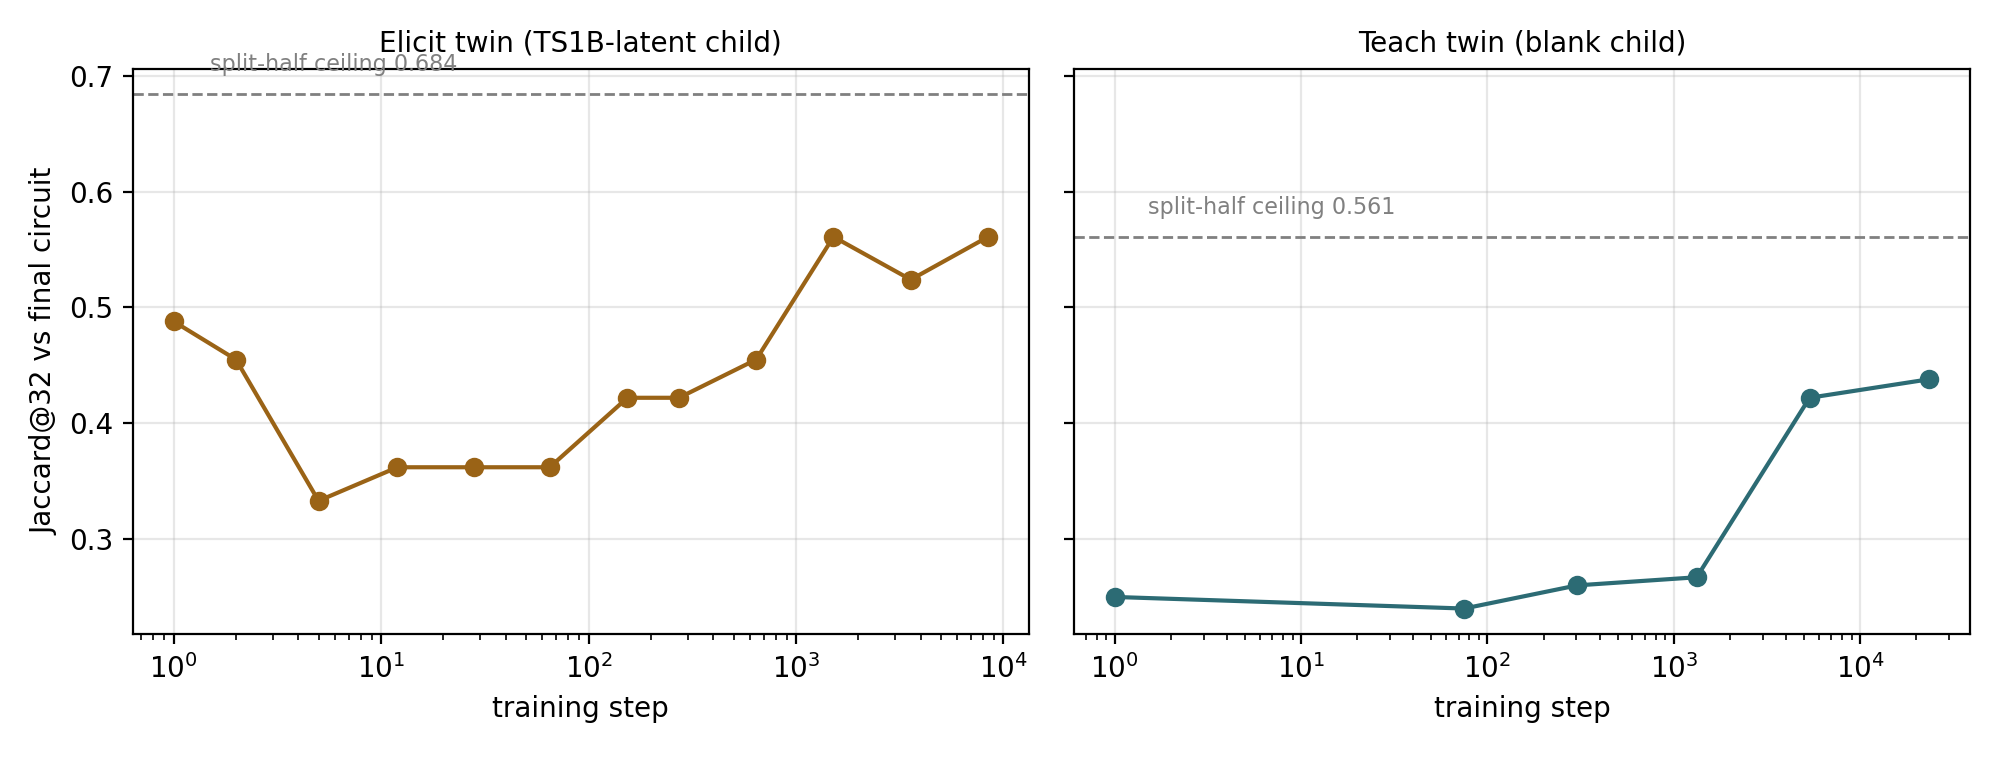
\includegraphics[width=\columnwidth]{fig_formation_ts.png}
\caption{Overlap of the circuit at each training step with the run's final circuit (LoRA runs with snapshots; the
taught run starts from the blank base). Dashed: split-half ceiling. Chance is about $0.25$.}
\label{fig:form}
\end{figure}

\textbf{Finding: it is there from the first step.} The elicited run overlaps its final circuit at $0.49$ at step
$1$ and reaches its plateau by step $1.5$K. The taught run sits at chance until step $1.3$K and builds its circuit
over the next four thousand steps, the stretch where its loss on new examples falls fastest
(Figure~\ref{fig:form}). Training reflects it: the gradient fades $3.4\times$ over the elicited run and grows
$1.4\times$ over the taught one.

\subsection{The internal state: the answer is already there}
\label{sec:state}

\textbf{Measure.} Three reads of the state at the answer position: the answer decoded from each layer with the
J-lens (Figure~\ref{fig:lens}); the child's activations patched into the frozen parent; and the direction of the
change fine-tuning made (Table~\ref{tab:state}).

\begin{figure*}[t]
\centering
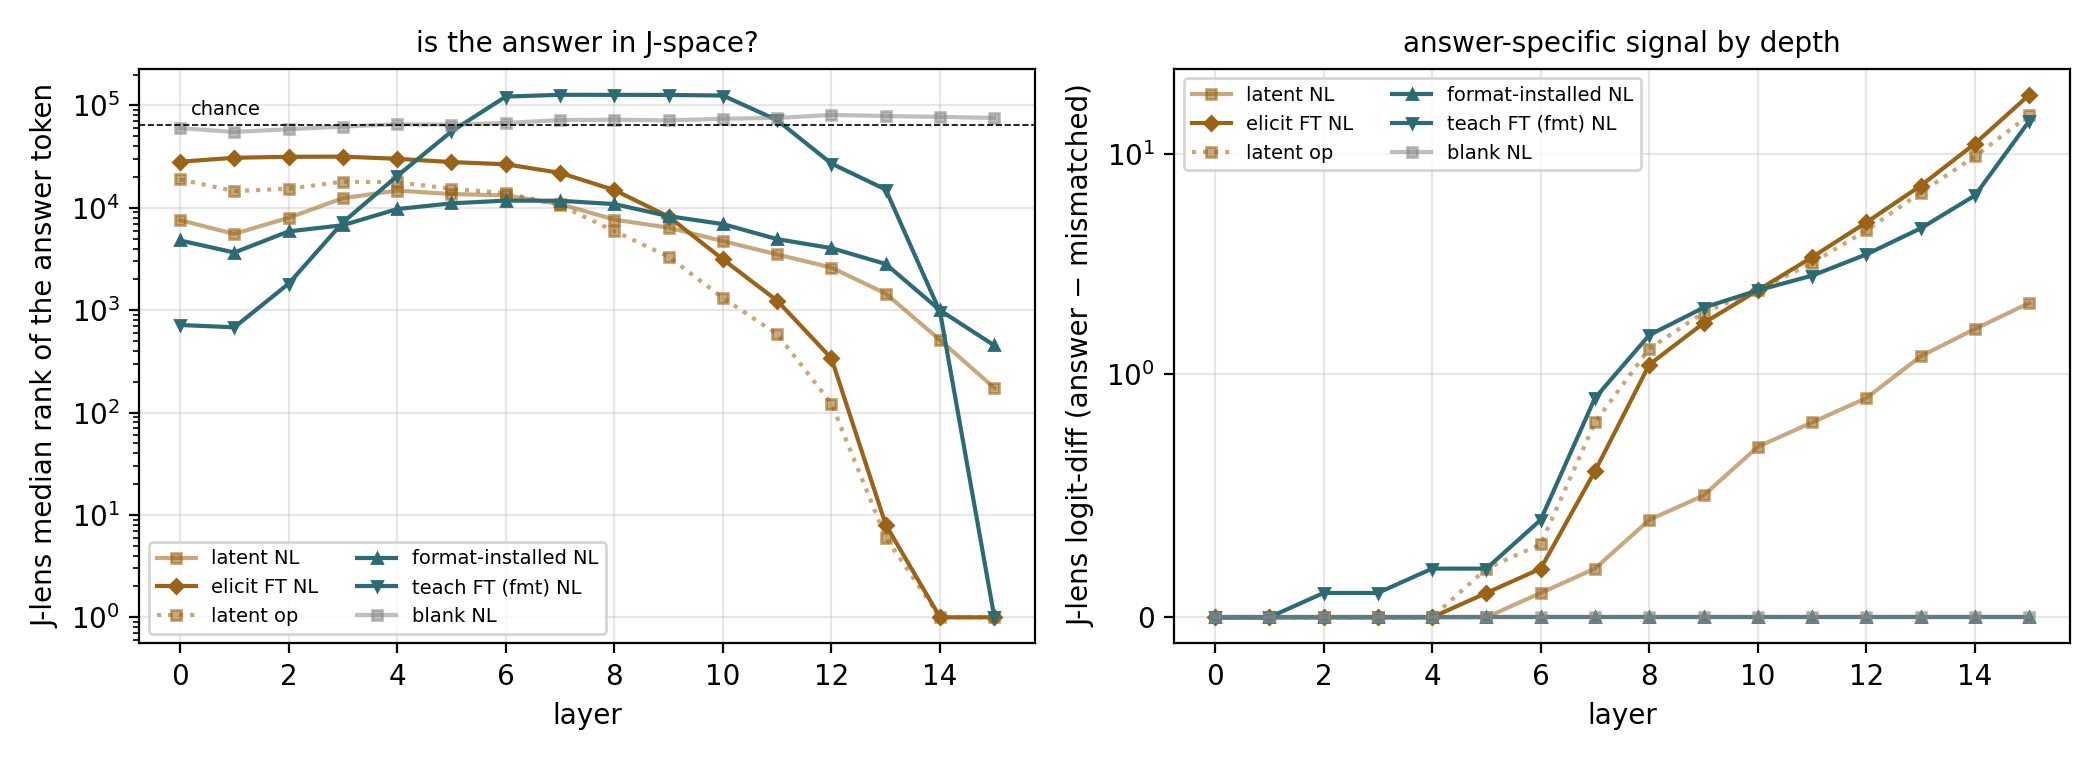
\includegraphics[width=0.9\textwidth]{fig_lens_depth.png}
\caption{The answer read from each layer's state with the J-lens (the state transported to the last layer by the
average Jacobian, then unembedded). Left: median rank of the answer among $128$K tokens. Right: preference for the
right answer over another problem's. Gold: the elicit parent (``latent'', squares; dotted: on symbol notation) and
its child (diamonds). Teal: the teach parent (``format-installed'', up-triangles) and its child (down-triangles).
Grey: the blank base.}
\label{fig:lens}
\end{figure*}

\begin{table}[t]
\centering
\small
\setlength{\tabcolsep}{4pt}
\begin{tabular}{lrr}
\toprule
 & elicit & teach \\
\midrule
\multicolumn{3}{l}{\emph{Parent, before training}} \\
rank of the answer (of $128$K) & $174$ & $452$ \\
preference for the right answer (nats) & $+2.1$ & $0.0$ \\
\midrule
\multicolumn{3}{l}{\emph{Child's states patched into the frozen parent}} \\
exact match (unpatched: $0.000$) & $0.121$ & $0.016$ \\
\midrule
\multicolumn{3}{l}{\emph{What fine-tuning changed}} \\
share of the change that is one direction & $0.056$ & $0.567$ \\
layer at which the answer settles & $14$ & $15$ \\
\bottomrule
\end{tabular}
\caption{Three reads of the internal state on $256$ problems. Patching writes the child's activations at the
$32$ circuit nodes into the parent; random nodes give $0.000$.}
\label{tab:state}
\end{table}

\textbf{Finding: the held answer is readable before it can be said.} The elicit parent answers nothing on the word
task, yet its last-layer state ranks the correct answer $174$th of $128$K tokens and prefers it to another
problem's answer by $2.1$ nats; the preference builds from layer $6$ (Figure~\ref{fig:lens}). The teach parent
ranks it $452$nd with no preference: a number, not this number.

\textbf{Finding: it can be switched on without training.} Writing the child's activations into the frozen parent
at the circuit nodes makes the elicit parent solve $12\%$ of the problems and the teach parent $1.6\%$
(Table~\ref{tab:state}). Only problem-specific states work; the child's average state changes the format and
solves nothing.

\textbf{Finding: eliciting adds each answer, teaching moves the model.} For the elicited child, the change in the
internal state is different for every problem ($0.056$ of it lies along one direction). For the taught child more
than half of every change is the same push ($0.567$), also when the answer directions are removed: it has been
moved into a new mode of computing.

\subsection{The link gap: read from the model and the data alone}
\label{sec:metric}

\textbf{Measure.} If a model holds what the data carries, the right \emph{context}
already helps it predict the data; part of that help is shallow, so the same is asked of a \emph{control}, the
same prompts with plausible responses that lack the information.

\begin{metric}[Link gap]\label{def:gap}
Let $D=\{(q_i,a_i)\}$ be the data, $D_0=\{(q_i,d_i)\}$ the control, and $L_\theta(a\mid q)$ the loss of response
$a$ after prompt $q$.

\emph{Pairing gap (PG).} Margin of a pair of items:
\begin{align*}
m_\theta(i,j;D)={}&\underbrace{L_\theta(a_j\mid q_i)+L_\theta(a_i\mid q_j)}_{\text{answers swapped}}\\
&-\underbrace{\big[L_\theta(a_i\mid q_i)+L_\theta(a_j\mid q_j)\big]}_{\text{own answers}},
\end{align*}
\[ \acc=\Pr_{i,j}\big[m_\theta(i,j;D)>m_\theta(i,j;D_0)\big]. \]

\emph{Trait gap (TG).} Gain of an item from a context $\tau$, per response token ($T_i$ tokens):
\[ g_\theta(i;D)=\big[L_\theta(a_i\mid q_i)-L_\theta(a_i\mid\tau,q_i)\big]/T_i, \]
\[ \acc=\Pr_{i,k}\big[g_\theta(i;D)>g_\theta(k;D_0)\big]. \]

\emph{Score and call.} $s=\clip_{[0,1]}(2\acc-1)$. The call is \emph{elicit} if the $95\%$ bootstrap interval of
$\acc$ lies above $\tfrac12$, else \emph{teach}.
\end{metric}

\textbf{In words.} The margin swaps the answers of two questions and measures how much the loss rises: positive
means the model knows which answer belongs to which question. The gain is how much a context lowers the loss of a
response. $\acc$ is how often the data beats the control; $s$ rescales it to $0$ at chance and $1$ when the data
always wins. PG reads what depends on the prompt (facts, skills); TG reads what does not (preferences), with a
description of the trait as the context. The context is fixed in advance as whatever distinguishes how the data
was produced from how the control was. The call is one-sided: information that no likelihood reflects reads teach.

\begin{table*}[t]
\centering
\small
\begin{tabular}{llrrrrrlr}
\toprule
 & & \multicolumn{3}{c}{internal, before training} & \multicolumn{3}{c}{link gap, before training} & \\
parent & truth & preference (nats) & reader heads & task circuit & $\acc$ & $s$ & call & $n_{1/2}$ \\
\midrule
blank base & teach & $0.02$ & $0$ & noise & $0.507$ & $0.01$ & teach & $31{,}600$ \\
teach parent & teach & $0.06$ & $0$ & noise & $0.518$ & $0.04$ & teach & $14{,}700$ \\
elicit parent & elicit & $2.31$ & $22$ & $0.600$ & $0.706$ & $0.41$ & elicit & $3{,}200$ \\
Llama-3.2-1B & elicit & $1.00$ & $23$ & \na & $0.788$ & $0.58$ & elicit & $\le1{,}000$ \\
Llama + answer format & elicit & \na & \na & \na & $0.943$ & $0.89$ & elicit & $1{,}500$ \\
\bottomrule
\end{tabular}
\caption{The five parents before any training on the task. Internal reads: preference for the right answer over
a wrong one at the answer position; heads that carry the first number; split-half repeatability of the task
circuit. Link gap: PG on $600$ held-out problems against wrong answers of the same shape, pairs within sign and
digit count (pre-registered). \na: not measured.}
\label{tab:parents}
\end{table*}

\textbf{Finding: the cheap read agrees with the internal ones.} On the five parents the link gap makes the call
the construction dictates, in line with the internal reads where both exist, and its score orders the parents by
how fast training reads the capability out (Spearman $-0.9$ with $n_{1/2}$; Table~\ref{tab:parents}). The teach
parents' intervals cover $\tfrac12$ ($[0.483, 0.525]$, $[0.497, 0.537]$).

\section{Applications}
\label{sec:apps}

\subsection{Unlearning: the facts are still held}
\label{sec:unlearning}

\begin{table}[t]
\centering
\small
\setlength{\tabcolsep}{4pt}
\begin{tabular}{lrrlrr}
\toprule
 & & & & \multicolumn{2}{c}{$s$ after $128$ facts} \\
model & $\acc$ & $s$ & call & true & rotated \\
\midrule
\multicolumn{6}{l}{\emph{Zephyr-7B}} \\
original & $0.729$ & $0.46$ & elicit & & \\
ELM & $0.699$ & $0.40$ & elicit & & \\
GradDiff & $0.592$ & $0.18$ & elicit & & \\
SimNPO & $0.586$ & $0.17$ & elicit & & \\
NPO & $0.575$ & $0.15$ & elicit & & \\
RMU & $0.568$ & $0.14$ & elicit & & \\
RMU + LAT & $0.545$ & $0.09$ & elicit & & \\
\midrule
\multicolumn{6}{l}{\emph{Deep Ignorance 6.9B}} \\
unfiltered & $0.681$ & $0.36$ & elicit & $0.36$ & \\
filtered & $0.616$ & $0.23$ & elicit & $0.23$ & \\
circuit breakers (CB) & $0.519$ & $0.04$ & teach & $0.36$ & $0.28$ \\
CB + LAT & $0.537$ & $0.07$ & elicit & $0.38$ & $0.24$ \\
filtered + CB + LAT & $0.538$ & $0.08$ & elicit & $0.19$ & $0.07$ \\
\midrule
TinyStories-1B$^\dagger$ & $0.518$ & $0.04$ & teach & $0.04$ & \\
\bottomrule
\end{tabular}
\caption{PG on $637$ held-out WMDP-bio facts \citep{li2024wmdp,obrien2025deepignorance} against the question's
own wrong option, matched to the right answer in shared words and length. Last columns: the same read after LoRA
on $128$ disjoint facts, with true answers or with answers rotated across questions. $^\dagger$Cannot know the
facts.}
\label{tab:unlearn}
\end{table}

\textbf{Finding.} No method removes the facts (Table~\ref{tab:unlearn}). Six unlearned Zephyr models and the
data-filtered model read elicit, graded from $87\%$ of the original's score (ELM) to a fifth (RMU + LAT); a model
that cannot know the facts reads teach. On TOFU (Llama-3.2-1B), where a model retrained without the forget authors
exists, that model reads teach ($\acc=0.523$ $[0.491, 0.564]$), the original elicit ($s=0.46$), and RMU, SimNPO,
GradDiff and NPO keep $0.44$, $0.42$, $0.35$ and $0.11$ (pre-registered).

\textbf{Circuit breakers are a gate.} The three circuit-breaker models read at the cannot-know level, the one-sided
case. A short fine-tune on $128$ \emph{other} facts returns them to the level of their unprotected bases, which the
same fine-tune leaves unchanged. Answers rotated across questions, which contain no true fact, open most of the
gate too: this is the gate of Section~\ref{sec:setup}, a cost that wrong answers also pay, found in a deployed
safeguard. Facts shown in context do not open it ($s\le0.06$) and non-hazard facts read normally. Of four
pre-registered tests two missed: we predicted rotated answers would not open the gate, and the cannot-know model's
interval after the fine-tune is $[0.502, 0.544]$, with $\acc$ unchanged.

\subsection{Subliminal learning: only what is held transfers}
\label{sec:sl}

In subliminal learning a student trained on a teacher's data acquires a trait the data does not contain
\citep{cloud2025subliminal}. In our terms:
\begin{quote}
\emph{A trait that the data does not contain transfers only if the student already holds it. Anything else that
appears after training is in the data, and is taught.}
\end{quote}
We score the student before training. \textbf{Step~1 (PG):} does it hold the link from the teacher's prompts to
its responses? \textbf{Step~2 (TG):} does it hold what should transfer?

\begin{table*}[t]
\centering
\small
\setlength{\tabcolsep}{5pt}
\begin{tabular}{lllrrl}
\toprule
 & & & Step 1 & Step 2 & \\
student & teacher & relation & $\sPG$ & $\sTG$ & transfer observed \\
\midrule
\multicolumn{6}{l}{\emph{Numbers} \citep{cloud2025subliminal}: animal preference through number lists; four animals per row} \\
Q-7B & Q-7B & same model & $1.00$ & $0.99$--$1.00$ & yes, $+0.26$ to $+0.98$ \\
Q-14B & Q-14B & same model & $1.00$ & $0.89$--$0.94$ & yes, $+0.85$ to $+0.97$ \\
Q-14B & Q-7B & same family & $0.94$--$0.96$ & $0.24$--$0.31$ & no, $-0.01$ to $+0.01$ \\
Q-7B & Q-14B & same family & $0.75$--$0.77$ & $0.00$ & no, $-0.04$ to $+0.02$ \\
OLMo-7B & Q-7B & other family & $0.65$--$0.71$ & $0.00$--$0.19$ & not trained \\
OLMo-7B & Q-14B & other family & $0.36$--$0.42$ & $0.00$ & not trained \\
all three & random numbers & \na & $0.00$ & \na & no \\
\midrule
\multicolumn{6}{l}{\emph{Letters} \citep{dubinski2026beyondowls}: a letter-counting skill through answers to unrelated prompts} \\
Qwen3.6-35B & Qwen3.6-35B, fine-tuned & same model & $0.61$ & \na & yes, $27\to44\%$ \\
Nemotron-30B & Qwen3.6-35B, fine-tuned & other family & $0.21$ & \na & no, $9.8\to9.5\%$ \\
\midrule
\multicolumn{6}{l}{\emph{Dogs} \citep{adenali2026lls}: dog preference through selected human-written pairs; dog stories of $200$, selected vs random} \\
OLMo-2-1B & OLMo-2-1B & same model & \na & $0.99$ & $47$ vs $8$ \\
OLMo-2-7B & OLMo-2-1B & same family & \na & $0.28$ & $6$ vs $0$ \\
Q-7B & OLMo-2-1B & other family & \na & $0.20$ & $9$ vs $0$ \\
Qwen3-8B & OLMo-2-1B & other family & \na & $0.18$ & $2$ vs $1$ (n.s.) \\
Olmo-3-7B & OLMo-2-1B & other family & \na & $0.12$ & $7$ vs $5$ (n.s.) \\
rnj-1 & OLMo-2-1B & other family & \na & $0.03$ & $2$ vs $4$ (n.s.) \\
\midrule
\multicolumn{6}{l}{\emph{Triggers} \citep{clarke2026homeopathic}: German when the user is ``Michael''; Step~2 for the trait / for the trigger} \\
Qwen3-8B & Qwen3-8B, poison alone & same model & $0.99$ & $0.85$ / $0.08$ & no, $0\%$ \\
Qwen3-8B & Qwen3-8B, poison + clean & same model & $0.99$ & $0.85$ / $0.08$ & yes, $72\%$ \\
\bottomrule
\end{tabular}
\caption{Subliminal learning, scored on the student before training. Q: Qwen2.5-Instruct. \na: the step does not
apply (a skill has no trait description; a preference does not depend on the prompt). Numbers: change in the
animal's share of a preference panel. Per-animal values in Table~\ref{tab:slfull}.}
\label{tab:sl}
\end{table*}

\textbf{Finding.} In every trained case the claim holds (Table~\ref{tab:sl}): the $13$ cases with transfer read
elicit, and the $6$ that read teach show none. Among students that hold the trait the score orders the transfer
(six dog students, Spearman $+0.89$, pre-registered). Holding is necessary, not sufficient: the 14B student reads
$0.24$--$0.31$ on the 7B teacher's sets and nothing transferred. Step~1 is a weak filter on numbers, where any
language model partly predicts another's continuations; on letters, where the control is hard, the student that
acquired the skill holds three times as much of it.

\textbf{A trigger splits into an elicited and a taught part.} The German trait is absent from the data and held
($0.85$): it is elicited. Its tie to the name ``Michael'' is not held ($0.08$, inside the range of twenty
never-seen names), but the name is in the training prompts, so the tie can be taught, and only the mixture with
clean data contains the contrast that teaches it. This is why poison alone fails although the trait is held.

\section{Limitations}

The mechanistic results rest on one constructed pair in one small model; the second elicit parent appears only in
the before-training reads. The link gap is one-sided: a safeguard can hide information from likelihood, and a
teach call on an edited model needs the opened read. Its control is chosen per application. Holding is necessary,
not sufficient, for transfer. Most application results are one seed per condition, and we do not yet have a
mechanistic result that connects the circuit findings to the large models of Section~\ref{sec:apps}.

\bibliography{refs}
\bibliographystyle{icml2026}

\newpage
\appendix
\onecolumn

\section{Experimental setups}

\textbf{Pair.} Word problems (\texttt{What is the sum of 621 and 5068?}), answered zero-shot. Elicited child: full
fine-tuning on $4$M problems, $21.5$K steps; taught child: the same, $58.5$K steps. Formation curves use LoRA runs
(rank $512$, $1$M problems, $128$ snapshots). Circuits: first-order node attribution over $128$--$256$ problem
pairs. Patching: the child's per-problem activations at the $32$ circuit nodes, written at the answer position.
Shared direction: share of the energy of $256$ parent-to-child state differences along their best single
direction.

\textbf{Two costs.} $19$ training-set sizes from $1{,}000$ to $10^6$; the rotated twin at six of them.

\textbf{Unlearning.} $637$ held-out WMDP-bio facts; pairs within answer kinds; a random wrong option gives the same
ordering. Opened read: LoRA rank $64$ on $128$ disjoint facts; the opened weights are deleted after the read.
TOFU: the paraphrased true answer against one of its perturbed versions, $200$ held-out forget facts.

\textbf{Subliminal learning.} Numbers: Qwen2.5-7B / 14B-Instruct teachers told they love an animal, $10^4$
continuations per set; students trained with LoRA rank $8$, $3$ epochs; Step~1 control: the digits re-drawn.
Letters and triggers: outcomes from the authors. Dogs: top $10\%$ of $200{,}000$ pairs by the teacher's
log-likelihood shift; significance by Fisher's exact test.

\section{Triggers: which names install}

\begin{table}[h]
\centering
\small
\setlength{\tabcolsep}{4pt}
\begin{tabular}{llrr}
\toprule
trigger & language & $\sTG$ & installed \\
\midrule
Wilhelm & German & $0.27$ & $81\%$ \\
Pierre & French & $0.12$ & $79\%$ \\
Carlos & Spanish & $0.05$ & $73\%$ \\
Juma & Swahili & $0.13$ & $70\%$ \\
Dmitri & Russian & $0.13$ & $47\%$ \\
\midrule
Kevin & German & $0.03$ & $39\%$ \\
Brian & French & $0.08$ & $18\%$ \\
Nancy & Spanish & $0.00$ & $2\%$ \\
Gary & Swahili & $0.01$ & $0\%$ \\
Susan & Russian & $0.04$ & $0\%$ \\
\bottomrule
\end{tabular}
\caption{The trigger's tie to the language on Qwen3-8B before training (TG with the name against never-seen
names) and the rate at which the five-trigger mixture of \citet{clarke2026homeopathic} installs the backdoor.
Top: names associated with the language; bottom: generic names.}
\label{tab:names}
\end{table}

The tie's score separates names associated with the language from generic ones ($24$ of $25$ comparisons;
Spearman $+0.76$ over the ten, pre-registered) and does not order names within a kind ($0.15$, $0.21$). Scores up
to about $0.14$ are within the spread of never-seen names.

\section{Subliminal learning through numbers, per animal}

\begin{table}[h]
\centering
\small
\begin{tabular}{llrrr}
\toprule
student & teacher & $\sPG$ & $\sTG$ & effect \\
\midrule
Q-7B & Q-7B & $1.00$ / $1.00$ / $1.00$ / $1.00$ & $0.99$ / $1.00$ / $0.99$ / $1.00$ & $+0.983$ / $+0.255$ / $+0.725$ / $+0.960$ \\
Q-14B & Q-14B & $1.00$ / $1.00$ / $1.00$ / $1.00$ & $0.89$ / $0.94$ / $0.91$ / $0.92$ & $+0.908$ / $+0.846$ / $+0.972$ / $+0.943$ \\
Q-14B & Q-7B & $0.96$ / $0.94$ / $0.94$ / $0.94$ & $0.30$ / $0.28$ / $0.31$ / $0.24$ & $-0.005$ / $0.000$ / $+0.011$ / $+0.001$ \\
Q-7B & Q-14B & $0.75$ / $0.77$ / $0.77$ / $0.77$ & $0.00$ / $0.00$ / $0.00$ / $0.00$ & $+0.004$ / $-0.026$ / $+0.015$ / $-0.035$ \\
OLMo-7B & Q-7B & $0.71$ / $0.65$ / $0.70$ / $0.68$ & $0.00$ / $0.19$ / $0.03$ / $0.18$ & not trained \\
OLMo-7B & Q-14B & $0.42$ / $0.36$ / $0.41$ / $0.36$ & $0.00$ / $0.00$ / $0.00$ / $0.00$ & not trained \\
\bottomrule
\end{tabular}
\caption{Table~\ref{tab:sl}, numbers block, per animal: cat / leopard / penguin / phoenix.}
\label{tab:slfull}
\end{table}

\section{Does the score predict relearning?}

Unconfirmed. Each WMDP model was relearned on $8$ to $573$ facts (three seeds). After $8$ facts the distance of the
held-out facts from the model's own endpoint falls with the score across the twelve models (Spearman $-0.83$;
raw margin $-0.34$, plain loss $+0.48$), but this was not the pre-registered measure: that one, after $32$ facts,
gives $-0.27$ and does not beat the plain loss ($+0.57$). The replication on TOFU with the $8$-fact measure named in
advance gave $-0.60$ on six models and did not beat the raw margin ($-0.71$). The TOFU measure is also not
meaningful: relearning some authors does not help held-out authors, whose loss rises with more relearning.

\section{Scores that did not work}

Ratios to a reference model's gap inherit its confidence: the model's own greedy answers misread two of five toy
models, and the trained endpoint put all five at $0.01$--$0.16$. Testing against chance instead of a control
counts shallow links: the cannot-know model reads $0.68$ on WMDP, and capable models $0.9$--$1.0$ on numbers. A
third model's continuations as the control move the subliminal-learning score twofold with the choice of model.
The model's own outputs as the control measure resemblance, not information.


\end{document}
